% ============================================================================
% Lecture 22 (B21): Deep Surrogate Models
% Deep Learning for Solving and Estimating Dynamic Models in Economics and Finance
% Course author: Simon Scheidegger
% ============================================================================

\documentclass[aspectratio=169,11pt]{beamer}

% ---------- Theme and colors ----------
\usecolortheme{dove}
\setbeamertemplate{navigation symbols}{}
\setbeamertemplate{footline}{%
  \hfill\usebeamerfont{page number in head/foot}%
  \usebeamercolor[fg]{normal text}%
  \insertframenumber\,/\,\inserttotalframenumber\kern1em\vskip4pt}
\setbeamerfont{frametitle}{size=\huge}

% ---------- Packages ----------
\usepackage[utf8]{inputenc}
\usepackage[T1]{fontenc}
\usepackage{amsmath,amssymb,amsfonts}
\usepackage{bm}
\usepackage{graphicx}
\usepackage{tikz}
\usetikzlibrary{shapes,arrows.meta,positioning,calc,fit,backgrounds,patterns,decorations.pathreplacing}
\usepackage{pgfplots}
\pgfplotsset{compat=1.18}
\usepackage{booktabs}
\usepackage{hyperref}
\usepackage{multicol}
\usepackage{xcolor}
\usepackage{algorithm}
\usepackage{algorithmic}
\usepackage{listings}
\usepackage{pifont}

% ---------- Listings style for Python ----------
\lstset{
    language=Python,
    basicstyle=\small\ttfamily,
    keywordstyle=\color{uzhblue}\bfseries,
    commentstyle=\color{uzhgreydark}\itshape,
    stringstyle=\color{darkgreen},
    showstringspaces=false,
    breaklines=true,
    frame=none,
    xleftmargin=0pt,
    aboveskip=4pt,
    belowskip=4pt,
    escapeinside={(*@}{@*)},
}

% ---------- Custom colors ----------
\definecolor{uzhblue}{rgb}{0,0,0.5}
\definecolor{uzhgreylight}{RGB}{236,238,241}
\definecolor{uzhgreydark}{RGB}{81,86,94}
\definecolor{harvardcrimson}{RGB}{153,0,0}
\definecolor{unil@blue}{RGB}{0,140,204}
\definecolor{unil@black}{RGB}{35,31,32}
\definecolor{darkgreen}{RGB}{0,100,0}
\definecolor{darkred}{RGB}{139,0,0}
\definecolor{softblue}{RGB}{70,130,180}
\definecolor{softorange}{RGB}{230,159,0}
\definecolor{softgreen}{RGB}{0,158,115}

% ---------- Set beamer colors ----------
\setbeamercolor{frametitle}{bg=uzhgreylight, fg=uzhblue}
\setbeamercolor{title}{fg=uzhblue}
\setbeamercolor{structure}{fg=uzhblue}
\setbeamercolor{block title}{bg=unil@blue, fg=white}
\setbeamercolor{block body}{bg=uzhgreylight}
\setbeamercolor{block title alerted}{bg=darkred,fg=white}
\setbeamercolor{block body alerted}{bg=red!5}
\setbeamercolor{block title example}{bg=darkgreen,fg=white}
\setbeamercolor{block body example}{bg=green!5}
\setbeamercolor{item}{fg=unil@black}
\setbeamercolor{normal text}{fg=unil@black}

% ---------- Emphasis and hyperlinks ----------
\newcommand{\emphc}[1]{\textcolor{harvardcrimson}{#1}}
\hypersetup{colorlinks,linkcolor=harvardcrimson,urlcolor=harvardcrimson}

% ---------- Math commands ----------
\newcommand{\x}{\bm{x}}
\newcommand{\w}{\bm{w}}
\newcommand{\bb}{\bm{b}}
\newcommand{\z}{\bm{z}}
\newcommand{\W}{\bm{W}}
\newcommand{\X}{\bm{X}}
\renewcommand{\a}{\bm{a}}
\newcommand{\R}{\mathbb{R}}
\newcommand{\E}[1]{\mathbb{E}\!\left[#1\right]}
\DeclareMathOperator*{\argmin}{arg\,min}
\DeclareMathOperator*{\argmax}{arg\,max}

% ---------- Title ----------
\title[Lecture 25 (B24)]{Lecture 25 (B24): Gaussian Processes for Dynamic Programming}
\subtitle{ASGP value-function iteration, active subspaces, parallelization, GPs vs DEQNs}
\author{Simon Scheidegger}
\institute{HEC, University of Lausanne}
\date{}
\begin{document}

% Custom command used in some "Finger Exercise" frame titles.
\providecommand{\exercisepause}{%
  \tikz[baseline=(X.base)]{\node[fill=darkgreen!80!black, text=white,
  rounded corners=2pt, inner sep=3pt, font=\scriptsize\bfseries](X){PAUSE};}}

{\setbeamercolor{background canvas}{bg=uzhgreylight}
\begin{frame}
\titlepage
\end{frame}
}

\section{GPs for Dynamic Programming}

% --- Section Divider ---
\begin{frame}{}
\vfill
\begin{center}
{\Huge \textcolor{uzhblue}{\textbf{Part IV}}}\\[12pt]
{\LARGE Gaussian Processes for Dynamic Programming}\\[8pt]
{\small Based on: Scheidegger \& Bilionis (2019), \emph{J.\ Comput.\ Sci.}\ 33, 68--82.}
\end{center}
\vfill
\end{frame}

% --- Slide: What is Dynamic Programming? (simple intro) ---
\begin{frame}{What is Dynamic Programming?}
\small
\textbf{Dynamic programming} (DP) is the core method for solving \emphc{sequential decision problems} under uncertainty---the backbone of macro, finance, and structural IO.

\vspace{0.4em}
\begin{columns}[T]
\column{0.48\textwidth}
\textbf{The idea:} An agent makes decisions over time to maximize total discounted utility:
\[
V(\x_0) = \max \sum_{t=0}^{\infty} \beta^t\, r(\x_t, \xi_t)
\]
subject to $\x_{t+1} \sim F(\cdot \,|\, \x_t, \xi_t)$.

\vspace{0.3em}
\textbf{Bellman's principle of optimality:}
\[
V(\x) = \max_\xi \bigl\{ r(\x, \xi) + \beta\, \E{V(\x_{t+1})} \bigr\}
\]
Solve this \emphc{one equation} instead of the infinite-horizon problem.

\column{0.48\textwidth}
\textbf{Why DP matters:}
\begin{itemize}\itemsep1pt
    \item Asset pricing, consumption--savings
    \item Growth theory, capital accumulation
    \item Labor: job search, human capital
    \item Climate: optimal carbon taxation
\end{itemize}

\vspace{0.2em}
\textbf{Challenge:} Bellman equation on a \emphc{high-dimensional state space}---the curse of dimensionality.
\end{columns}
\end{frame}

% --- Slide: The Stochastic Growth Model ---
\begin{frame}{Example: The Stochastic Optimal Growth Model}
\small
Workhorse testbed for computational macro (cf.\ Days 2--3). Model with $D$ sectors:

\vspace{0.2em}
\begin{columns}[T]
\column{0.48\textwidth}
\begin{itemize}\itemsep0pt
    \item State: $\bm{k} = (k_1, \ldots, k_D)$
    \item Controls: consumption $\bm{c}$, labor $\bm{l}$, investment $\bm{i}$
    \item Production: $f(k_j, l_j) = A k_j^\psi l_j^{1-\psi}$
    \item Shocks: $\epsilon_{t,j} \sim \mathcal{N}(0, \sigma^2)$
    \item $k_{j}^+ = (1-\delta) k_j + i_j$
\end{itemize}

\vspace{0.2em}
$D$ ranges from 1 (textbook) to \emphc{500}.

\column{0.48\textwidth}
\textbf{Bellman equation:}
\[
V(\bm{k}) = \max_{\bm{c}, \bm{l}} \bigl\{ u(\bm{c}, \bm{l}) + \beta\, \E{V(\bm{k}^+)} \bigr\}
\]

\textbf{Challenge:} approximate $V$ on $\R^D$ at each VFI step. Grid methods fail for $D > 20$. \emphc{GPs as interpolation} $\Rightarrow$ arbitrary geometries, scales to 500D.
\end{columns}

\vspace{0.3em}
\begin{block}{Hands-on}
\small \texttt{04\_GP\_Value\_Function\_Iteration.ipynb} --- solves the $D=1$ case with GP-based VFI.
\end{block}
\end{frame}

% --- Slide: Key Idea ---
\begin{frame}{The Key Idea: GP as Value Function Surrogate}
\scriptsize
\begin{columns}[T]
\column{0.52\textwidth}
At each VFI step $s$:

\vspace{0.2em}
\begin{enumerate}\itemsep1pt
    \item Generate $n^s$ training inputs $\X$ in the state space
    \item Evaluate Bellman: $t_i^s = (TV^{s-1})(\x^{(i)})$
    \item Learn GP surrogate $V_{\text{surr}}$ from $\{\X, \bm{t}\}$
    \item Set $V^s = V_{\text{surr}}$ (posterior mean)
    \item Error: $\eta^s = \|V^s - V^{s-1}\|_\infty/\Delta_V$
\end{enumerate}

\vspace{0.2em}
GP posterior mean $\to$ next iterate; GP posterior \emphc{variance} $\to$ free uncertainty bounds at every step.

\column{0.45\textwidth}
\textbf{Why GPs instead of grids?}

\vspace{0.2em}
\begin{itemize}\itemsep1pt
    \item Work on \emphc{arbitrary geometries}---no tensor-product structure
    \item Training points \emphc{adaptively chosen}---concentrate near steep gradients
    \item Built-in \emphc{interpolation uncertainty}
    \item Non-converging points can be \emphc{discarded}---impossible with grids
\end{itemize}

\vspace{0.2em}
\begin{block}{Recall}
\tiny
Same GP posterior from Part~II, now applied iteratively inside a DP algorithm.
\end{block}
\end{columns}

\vspace{0.1em}
{\tiny \textbf{Origin:} GPDP — Deisenroth, Rasmussen \& Peters (2009, \emph{Neurocomputing}); economics/high-dim extension — Scheidegger \& Bilionis (2019, \emph{JoCS}).}
\end{frame}

% --- Slide: Algorithm ---
\begin{frame}[fragile]{Algorithm: ASGP Value Function Iteration}
\tiny
\begin{algorithmic}[1]
\STATE \textbf{Input:} Initial guess $V_{\text{next}}$, tolerance $\bar{\eta}$
\WHILE{$\eta > \bar{\eta}$}
    \STATE Generate $n^s$ training inputs $\X = \{\x^{(i)}\} \in [\underline{\bm{k}}, \bar{\bm{k}}]^D$
    \FOR{$\x^{(i)} \in \X$}
        \STATE Bellman target: $t_i = (TV_{\text{next}})(\x^{(i)})$; \quad policy: $\xi_j(\x^{(i)}) \in \argmax TV(\x^{(i)})$
    \ENDFOR
    \STATE Learn surrogate $V_{\text{surr}}$ with ASGP (or GP) from $\{\X, \bm{t}\}$
    \STATE Error: $\eta = \|V_{\text{surr}} - V_{\text{next}}\|_\infty$; \quad $V_{\text{next}} \leftarrow V_{\text{surr}}$
\ENDWHILE
\STATE \textbf{Output:} $V$, policy functions $\xi^* = (\xi_1^*, \ldots, \xi_{3D}^*)$
\end{algorithmic}

\vspace{0.3em}
{\scriptsize \textbf{Key:} Training set $\X$ can be \emphc{adaptively steered}---non-converging points excluded, new points added. Impossible with grids.}
\end{frame}

% --- New slide: Cheap BAL inside the VFI loop ---
\begin{frame}{Cheap BAL Inside the VFI Loop}
\textbf{Goal of acquisition.} Uniform interpolation accuracy of $V$, not optimization $\Rightarrow$ pure exploration.

\medskip
\textbf{Acquisition function.} Posterior standard deviation only:
\[
\x^{\text{next}} \in \argmax_{\x \in \mathcal{X}^{\text{cand}}} \sigma_{\text{GP}}^s(\x)
\quad \text{(no UCB, no EI).}
\]

\medskip
\textbf{Recipe.}
\begin{itemize}\itemsep0pt
  \item Every $N$ VFI iterations, score a Latin-hypercube candidate set
  \item Pick top $n_{\text{add}}$ by $\sigma_{\text{GP}}$, with min-spacing constraint to avoid clustering
  \item Evaluate Bellman operator at new points (parallel) and append to $\mathcal{D}^s$
\end{itemize}

\medskip
\textbf{Why pure exploration here.} A UCB-style acquisition would chase high-value states; we instead want $\sigma_{\text{GP}}$ small \emphc{everywhere} so the approximate Bellman operator stays close to a contraction.

\medskip
{\scriptsize Notebook 04 ($N=12$, $n_{\text{add}}=2$): active design beats naive LHS on both Bellman residual and LOO-RMSE.}
\end{frame}

% --- Slide: Active Subspaces ---
\begin{frame}{Active Subspaces: Breaking the Curse of Dimensionality}
\scriptsize
Standard GPs fail for $D \gtrsim 10$ (Euclidean distance uninformative). \emphc{Active Subspaces} (AS) find a low-dim manifold of maximal response variation.

\vspace{0.2em}
\begin{columns}[T]
\column{0.48\textwidth}
\textbf{Idea:} $f(\x) \approx h(\W^T\x)$, $\W \in \R^{D \times d}$, $d \ll D$.

\vspace{0.2em}
\textbf{Finding $\W$:}
\begin{enumerate}\itemsep0pt
    \item Collect gradients $\bm{g}^{(i)} = \nabla f(\x^{(i)})$
    \item $\bm{C}_N = \frac{1}{N}\sum \bm{g}^{(i)} (\bm{g}^{(i)})^T$
    \item SVD: $\bm{C}_N = \bm{V}\bm{\Lambda}\bm{V}^T$; find \emphc{sharp drop} in $\lambda_i$
    \item $\W = [\bm{v}_1, \ldots, \bm{v}_d]$ (top $d$ eigenvectors)
\end{enumerate}

\column{0.48\textwidth}
\textbf{The ASGP pipeline:}

\vspace{0.3em}
\begin{center}
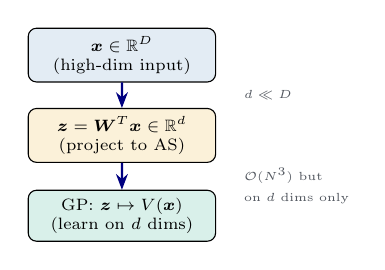
\begin{tikzpicture}[
    arr/.style={-{Stealth[length=2mm]}, thick, uzhblue},
    box/.style={draw, rounded corners=3pt, minimum width=2.8cm,
                minimum height=0.65cm, align=center, font=\scriptsize},
    scale=0.85, transform shape
]
    \node[box, fill=softblue!15] (hi) at (0,3) {$\x \in \R^D$\\(high-dim input)};
    \node[box, fill=softorange!15] (proj) at (0,1.8) {$\z = \W^T\x \in \R^d$\\(project to AS)};
    \node[box, fill=softgreen!15] (gp) at (0,0.6) {GP: $\z \mapsto V(\x)$\\(learn on $d$ dims)};
    \draw[arr] (hi) -- (proj);
    \draw[arr] (proj) -- (gp);
    \node[font=\tiny, text=uzhgreydark, anchor=west] at (1.7,2.4) {$d \ll D$};
    \node[font=\tiny, text=uzhgreydark, anchor=west] at (1.7,1.2) {$\mathcal{O}(N^3)$ but};
    \node[font=\tiny, text=uzhgreydark, anchor=west] at (1.7,0.85) {on $d$ dims only};
\end{tikzpicture}
\end{center}

\vspace{0.2em}
In the growth model, AS dim is typically $d = 1$, even when $D = 500$ $\Rightarrow$ \emphc{tractable}.
\end{columns}

\vspace{0.1em}
{\tiny \textbf{Hands-on:} \texttt{05\_Active\_Subspace\_2D}, \texttt{06\_..\_10D}, \texttt{07\_..\_Nonlinear} --- AS construction and ASGP vs GP comparison.}
\end{frame}

% --- Slide: When linear AS breaks ---
\begin{frame}{When the Active Manifold is Curved}
\scriptsize
Linear AS assumes the important directions are \emphc{linear} combinations of inputs: $f(\x) \approx h(\W^T \x)$.  If $f$ depends on a \emphc{nonlinear aggregate} of its inputs, the linear projection has to carry every direction that enters the aggregate -- not the aggregate itself.

\vspace{0.3em}
\begin{columns}[T]
\column{0.48\textwidth}
\textbf{Radial-ridge example} ($D = 20$):
\[
 y(\xi) \;=\; \exp\!\Bigl(-\bigl[(w_1^\top\xi)^2 + (w_2^\top\xi)^2\bigr]\Bigr).
\]
\begin{itemize}\itemsep0pt
  \item $C = \E[\nabla y\, \nabla y^\top]$ has \emphc{two} nonzero eigenvalues.
  \item Linear AS must pick $d_{\mathrm{lin}} = 2$.
  \item Yet the true intrinsic coordinate is the \emphc{scalar} $r^2 = (w_1^\top\xi)^2 + (w_2^\top\xi)^2$ -- one dimension.
\end{itemize}

\vspace{0.2em}
\textbf{Symptoms of curvature:}
\begin{itemize}\itemsep0pt
  \item Spectral gap ambiguous; $\lambda_i$ drops slowly.
  \item ASGP accuracy plateaus early as $d$ grows.
  \item Physics suggests thresholds, ridges, radial coords.
\end{itemize}

\column{0.48\textwidth}
\begin{center}
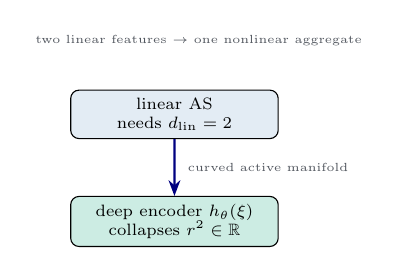
\begin{tikzpicture}[
    box/.style={draw, rounded corners=3pt, minimum width=3.1cm,
                minimum height=0.6cm, align=center, font=\scriptsize},
    arr/.style={-{Stealth[length=2mm]}, thick, uzhblue},
    scale=0.85, transform shape
]
    \node[box, fill=softblue!15]   (lin) at (0, 2.2) {linear AS\\needs $d_{\mathrm{lin}} = 2$};
    \node[box, fill=softgreen!20]  (nl)  at (0, 0.6) {deep encoder $h_\theta(\xi)$\\collapses $r^2 \in \R$};
    \draw[arr] (lin) -- node[right=2pt, font=\tiny, text=uzhgreydark]{curved active manifold} (nl);
    \node[font=\tiny, text=uzhgreydark, anchor=west] at (-2.2, 3.3) {two linear features $\to$ one nonlinear aggregate};
\end{tikzpicture}
\end{center}

\vspace{0.2em}
\textbf{Fix:} replace the linear projection $\W^T \x$ by a \emphc{learned nonlinear encoder} and jointly train a link function (Tripathy \& Bilionis, 2018).
\end{columns}

\vspace{0.1em}
{\tiny \textbf{Hands-on:} \texttt{09\_Deep\_Active\_Subspace\_Ridge} -- validates that deep AS recovers $d_{\mathrm{nl}} = 1$ on the radial ridge.}
\end{frame}

% --- Slide: Deep AS (Tripathy-Bilionis) ---
\begin{frame}{Deep Active Subspaces (Tripathy \& Bilionis, 2018)}
\scriptsize
Parametrize the surrogate as $\hat f(\xi) = g\bigl(h_\theta(\xi)\bigr)$, with \emphc{encoder} $h_\theta: \R^D \to \R^d$ and \emphc{link} $g_\theta: \R^d \to \R$ both small MLPs.  Setting $h_\theta(\xi) = U_m^\top \xi$ recovers the linear-AS ansatz, so the nonlinear encoder generalizes it.

\vspace{0.3em}
\begin{columns}[T]
\column{0.50\textwidth}
\textbf{Three design choices:}
\begin{enumerate}\itemsep1pt
  \item \textbf{Widths} decay exponentially
  $d_k = \lceil D \exp(\eta_{\mathrm{w}} k)\rceil$, $\eta_{\mathrm{w}} = \tfrac{1}{L}\log(d/D)$.
  \item \textbf{Swish activation} $\sigma(z) = z/(1 + e^{-z})$ (smooth, non-saturating).
  \item \textbf{Elastic-net loss}
  $\mathcal L = \tfrac{1}{N}\sum(\hat f - y_i)^2 + \lambda_1\|\theta\|_1 + \lambda_2\|\theta\|_2^2$.
\end{enumerate}

\vspace{0.3em}
\textbf{Gradient-free.} Learned from $(\xi_i, y_i)$ alone -- no $\nabla f$ samples, no orthogonality constraint.

\vspace{0.2em}
\textbf{Choosing $d$.} No spectral gap; use a \emphc{validation-MSE elbow} across $d = 1, 2, 3, \ldots$

\column{0.46\textwidth}
\begin{center}
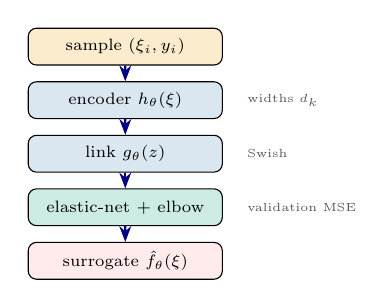
\begin{tikzpicture}[
    box/.style={draw, rounded corners=3pt, minimum width=2.9cm,
                minimum height=0.55cm, align=center, font=\scriptsize},
    arr/.style={-{Stealth[length=2mm]}, thick, uzhblue},
    scale=0.85, transform shape
]
    \node[box, fill=softorange!20] (sam)   at (0, 3.0) {sample $(\xi_i, y_i)$};
    \node[box, fill=softblue!20]   (enc)   at (0, 2.2) {encoder $h_\theta(\xi)$};
    \node[box, fill=softblue!20]   (lnk)   at (0, 1.4) {link $g_\theta(z)$};
    \node[box, fill=softgreen!20]  (eln)   at (0, 0.6) {elastic-net + elbow};
    \node[box, fill=red!8]         (sur)   at (0,-0.2) {surrogate $\hat f_\theta(\xi)$};
    \draw[arr] (sam) -- (enc);
    \draw[arr] (enc) -- (lnk);
    \draw[arr] (lnk) -- (eln);
    \draw[arr] (eln) -- (sur);
    \node[font=\tiny, text=uzhgreydark, anchor=west] at (1.7, 2.2) {widths $d_k$};
    \node[font=\tiny, text=uzhgreydark, anchor=west] at (1.7, 1.4) {Swish};
    \node[font=\tiny, text=uzhgreydark, anchor=west] at (1.7, 0.6) {validation MSE};
\end{tikzpicture}
\end{center}
\end{columns}

\vspace{0.1em}
{\tiny \textbf{Rule of thumb:} fit linear AS first; escalate to deep AS when (i) no gradients, (ii) ambiguous spectral gap, or (iii) $D \gg 10$ with curved manifold. \textbf{Hands-on:} \texttt{09\_..\_Ridge} (curved wins), \texttt{10\_..\_Borehole} (linear wins).}
\end{frame}

% --- Slide: Deep AS -- training recipe ---
\begin{frame}{Recipe: Fit a Deep Active Subspace}
\scriptsize
Self-contained recipe for the Tripathy-Bilionis architecture. All steps rely only on $(\xi_i, y_i)$ pairs -- no gradients, no Stiefel constraint, no kernel choice.

\vspace{0.2em}
\begin{columns}[T]
\column{0.54\textwidth}
\textbf{Algorithm.}
\begin{enumerate}\itemsep1pt
  \item \textbf{Sample} $(\xi_i, y_i)_{i=1}^N$; $80/20$ train/val split.
  \item \textbf{Standardize} inputs (unit variance), center outputs.
  \item For $d \in \{1, 2, 3, \ldots\}$:
    encoder $h_\theta\!: \R^D\!\to\!\R^d$ with widths $d_k = \lceil D e^{\eta_{\mathrm{w}} k}\rceil$, link $g_\theta\!: \R^d\!\to\!\R$ ($16$--$32$ units); train on
    $\mathcal L = \text{MSE}(\hat f, y) + \lambda_1\|\theta\|_1 + \lambda_2\|\theta\|_2^2$ with Adam + cosine LR.
  \item \textbf{Pick} $d$ at the \emph{validation-MSE elbow}.
  \item \textbf{Deploy}: $\hat f_\theta$ is the surrogate; $h_\theta(\xi)\!\in\!\R^d$ is a nonlinear \emphc{active coordinate} usable downstream (GP, sensitivity, optimization).
\end{enumerate}

\column{0.42\textwidth}
\textbf{Default hyperparameters:}
\vspace{0.1em}
\begin{center}
\renewcommand{\arraystretch}{1.05}
\tiny
\begin{tabular}{l l}
\toprule
encoder depth $L$ & $3$ \\
link hidden units & $16$--$32$ \\
activation & Swish ($\gamma = 1$) \\
optimizer & Adam, lr $5{\times}10^{-3}$ \\
schedule & cosine, $10^3$--$2{\cdot}10^3$ eps \\
$\lambda_1, \lambda_2$ & $10^{-5},\,10^{-4}$ \\
batch size & full batch if $N \lesssim 10^4$ \\
\bottomrule
\end{tabular}
\end{center}

\vspace{0.1em}
{\tiny \textbf{Samples:} $N \!\approx\! 50\,d_{\mathrm{nl}}$ to find the bottleneck, $\approx 200\,d_{\mathrm{nl}}$ for deployment.}
\end{columns}

\vspace{0.1em}
{\tiny \textbf{Sanity checks:} (i) validation curve monotone-then-flat in $d$; (ii) scatter of $h_\theta(\xi_i)$ vs.\ the first linear-AS coordinate shows whether the encoder has actually gone \emph{nonlinear}.}
\end{frame}

% --- Slide: Deep AS -- the elbow ---
\begin{frame}[shrink=5]{Reading the Validation-MSE Elbow}
\scriptsize
The spectral-gap heuristic of linear AS has no direct analogue for a neural encoder.  Tripathy \& Bilionis (2018) replace it by a \emphc{validation-MSE elbow}: train several latent dimensions and stop when extra capacity stops reducing held-out error.

\vspace{0.3em}
\begin{columns}[T]
\column{0.46\textwidth}
\textbf{How to read it.}
\begin{itemize}\itemsep1pt
  \item Plateau for $d \ge d_{\mathrm{nl}}$ $\Rightarrow$ intrinsic dim reached.
  \item Linear AS needs $d_{\mathrm{lin}} \ge d_{\mathrm{nl}}$ whenever the aggregate is nonlinear: the elbow sits \emphc{below} the spectral gap.
  \item If curves cross (as on the borehole) the function is nearly a ridge and linear AS + polynomial link is more data-efficient.
\end{itemize}

\vspace{0.2em}
\textbf{Three common shapes:}
\begin{itemize}\itemsep1pt
  \item \emphc{Sharp elbow at $d = 1$} -- classic radial / ridge target; deep AS wins.
  \item \emphc{Gradual decay} -- weak low-rank structure; more samples or richer encoder needed.
  \item \emphc{Flat} -- no low-dim structure; return to the original $D$-dimensional problem.
\end{itemize}

\column{0.50\textwidth}
\begin{center}
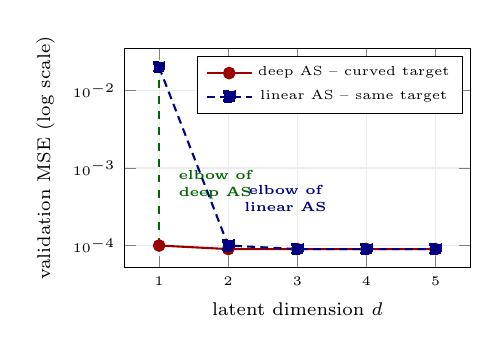
\begin{tikzpicture}[scale=0.95, transform shape]
\begin{axis}[
    width=6.2cm, height=4.5cm,
    xlabel={latent dimension $d$},
    ylabel={validation MSE (log scale)},
    ymode=log,
    xmin=0.5, xmax=5.5,
    xtick={1,2,3,4,5},
    ytick={1e-1,1e-2,1e-3,1e-4},
    grid=major, grid style={gray!15},
    legend style={font=\tiny, at={(0.98,0.97)}, anchor=north east},
    tick label style={font=\tiny},
    label style={font=\scriptsize},
]
\addplot[color=harvardcrimson, mark=*, thick]
  coordinates {(1,1e-4) (2,9e-5) (3,9e-5) (4,9e-5) (5,9e-5)};
\addlegendentry{deep AS -- curved target}
\addplot[color=uzhblue, mark=square*, thick, densely dashed]
  coordinates {(1,2e-2) (2,1e-4) (3,9e-5) (4,9e-5) (5,9e-5)};
\addlegendentry{linear AS -- same target}
\draw[dashed, darkgreen, thick]
  (axis cs:1,1e-4) -- (axis cs:1,2e-2);
\node[font=\tiny\bfseries, darkgreen, anchor=west]
  at (axis cs:1.15, 6e-4) {\shortstack{elbow of\\deep AS}};
\node[font=\tiny\bfseries, uzhblue, anchor=west]
  at (axis cs:2.1, 4e-4) {\shortstack{elbow of\\linear AS}};
\end{axis}
\end{tikzpicture}
\end{center}
{\tiny Stylized picture of the radial-ridge experiment (notebook \texttt{09}): deep AS flattens at $d = 1$, linear AS at $d = 2$.}
\end{columns}

\vspace{0.1em}
{\tiny \textbf{Operational test:} a drop of $<\!2\times$ in validation MSE between $d$ and $d+1$ is \emphc{not} worth paying the extra latent dimension for in most applications.}
\end{frame}

% --- Slide: Parallelization ---
\begin{frame}{Parallelization: Embarrassingly Parallel VFI}
\small
Bellman evaluations at $n^s$ training points are \emphc{independent} $\Rightarrow$ embarrassingly parallel.

\vspace{0.3em}
\begin{columns}[T]
\column{0.50\textwidth}
\textbf{MPI workflow:}
\begin{enumerate}\itemsep1pt
    \item \textbf{Broadcast} current $V_{\text{next}}$ to all workers
    \item \textbf{Evaluate:} each worker solves $n^s / n_{\text{cpu}}$ Bellman problems
    \item \textbf{Gather} training targets at master
    \item \textbf{Fit GP} surrogate (done once, centrally)
\end{enumerate}

\vspace{0.2em}
Communication cost negligible. Most time in parallelizable Bellman evaluations.

\column{0.47\textwidth}
\textbf{Scaling} (stochastic growth model):

\vspace{0.2em}
\scriptsize
\renewcommand{\arraystretch}{1.1}
\begin{tabular}{r r r}
\toprule
$D$ & Nodes & Total CPU h \\
\midrule
10 & 1 & 0.01 h \\
50 & 10 & 0.5 h \\
100 & 20 & 4 h \\
200 & 50 & 30 h \\
500 & 100 & $\sim$3700 h \\
\bottomrule
\end{tabular}

\vspace{0.3em}
\small
CPU time grows \emphc{sub-exponentially} ($<$2 days wall-clock for 500D with 100 nodes).
\end{columns}
\end{frame}

% --- Slide: Results ---
\begin{frame}[shrink=5]{Results: 1D to 500D Stochastic Growth}
\small
\begin{columns}[T]
\column{0.48\textwidth}
\textbf{Key results} (see Figs.~1--5 in the paper):
\begin{itemize}\itemsep3pt
    \item \textbf{1D:} Convergence in $\sim$70 VFI iterations; error $10^{-1} \to 10^{-5}$; GP CI bands negligible with just 10 training points
    \item \textbf{10D:} GP alone works; ASGP ($d=1$) equally accurate
    \item \textbf{50--500D:} ASGP converges to $10^{-4}$ normalized error; all dimensions converge in $\sim$70 iterations
\end{itemize}

\column{0.48\textwidth}
\textbf{Why this works:}
\begin{itemize}\itemsep3pt
    \item Active Subspace dimension is $d=1$ even for $D=500$ $\Rightarrow$ GP operates on 1D projected input
    \item Training set adaptively steered (drop non-converging points)
    \item Grid methods (Smolyak) cannot handle $D > 100$; ASGP \emphc{avoids the explicit grid-based curse} (does not eliminate all high-$d$ costs)
\end{itemize}
\end{columns}

\vspace{0.4em}
\begin{block}{Hands-on}
\textbf{Notebook:} \texttt{04\_GP\_Value\_Function\_Iteration.ipynb} --- solves the 1D growth model with GP-based VFI using scikit-learn. Shows convergence, value function with CI bands, and policy functions.
\end{block}
\end{frame}

% --- New slide: 2D GP-VFI in action ---
\begin{frame}{2D GP-VFI in Action}
\centering

\includegraphics[height=0.72\textheight,keepaspectratio]{fig/gp_vfi_2d_active_benchmark.pdf}

\smallskip
{\scriptsize Separable benchmark $V_2(k_1,k_2) = V^*(k_1) + V^*(k_2)$ with $\delta = 1$ closed form. Active design places points where $\sigma_{\text{GP}}$ is largest. (Notebook 04, cell~25.)}
\end{frame}

% --- Finger Exercise: GP-VFI ---
\begin{frame}{\exercisepause{} Finger Exercise: One Step of GP-Based VFI}
\begin{exampleblock}{Exercise (5 min)}
Consider a 1D growth model with $V(k) = \max_c \{ \log(c) + \beta\, V(k') \}$, $k' = k^{0.36} - c$, $\beta = 0.96$.  Suppose you have a GP trained on 3 points: $V(0.5) = -8.0$, $V(1.5) = -2.5$, $V(2.5) = 0.5$.
\begin{enumerate}
    \item At $k = 1.0$ (a new point not in the training set): the Bellman maximization yields $V^{\text{new}}(1.0) = -4.1$.  How does the GP posterior update when you add this observation?
    \item Does the GP posterior \emphc{variance} at $k = 1.0$ increase or decrease after adding this point?
    \item Why is it advantageous that training points can be added or removed freely, unlike grid-based methods?
\end{enumerate}
\end{exampleblock}
\end{frame}

\begin{frame}{Solution: One Step of GP-Based VFI}
\begin{block}{Answer}
\begin{enumerate}
    \item The GP is retrained on 4 points: $\{0.5, 1.0, 1.5, 2.5\}$.  The posterior mean $\mu(k)$ now interpolates through all 4 observations exactly (noiseless GP).  The posterior mean between existing points adjusts to accommodate the new observation.
    \item The posterior variance at $k = 1.0$ \emphc{decreases to zero} (the GP passes through the observation exactly).  Variance at nearby points also decreases.  Variance far from all training points remains large.
    \item \emphc{Flexibility:} If the Bellman operator at some point fails to converge (e.g., near a constraint), that point can simply be dropped.  On a grid, removing a point breaks the tensor-product structure.  This is a key advantage of GP-based VFI over grid-based methods.
\end{enumerate}
\end{block}
\end{frame}

% --- Slide: UQ and Ergodic Sets ---
\begin{frame}{UQ as a Byproduct \& Learning Ergodic Sets}
\scriptsize
\begin{columns}[T]
\column{0.48\textwidth}
\textbf{Uncertainty quantification:}

The GP posterior variance provides \emphc{free UQ} for the interpolated value function at every state point and VFI iteration. Policy uncertainty must be propagated through the maximization step.

\vspace{0.3em}
\textbf{Parameter uncertainty propagation:}
\begin{itemize}\itemsep1pt
    \item Add uncertain parameters as \emphc{pseudo-states}:\\
    $\tilde{S} = (\bm{k}, \gamma)$ where $\gamma \in [\underline{\gamma}, \bar{\gamma}]$
    \item Solve the model once on the extended state space
    \item Extract univariate effects: $\mathcal{M}_i(\chi_i) = \E{\mathcal{M}(\Theta) \mid \Theta_i = \chi_i}$
    \item Global sensitivity analysis (Sobol-style) in a \emphc{single computation}
\end{itemize}

\vspace{0.2em}
{\scriptsize This avoids the traditional approach of re-solving the model for each parameter value.}

\column{0.48\textwidth}
\textbf{Learning ergodic sets:}

Many economic models have \emphc{irregularly shaped} ergodic sets (ellipsoids, not hypercubes).

\vspace{0.3em}
\begin{enumerate}\itemsep2pt
    \item Solve model on a large domain initially
    \item Simulate the economy to generate capital paths $\{\bm{k}_t^+\}$
    \item Fit a \emphc{Bayesian Gaussian Mixture Model} to learn\\
    $\hat{\rho}_{\text{ergodic}}(\x)$
    \item Re-solve on the ergodic set only---sample training points from $\hat{\rho}_{\text{ergodic}}$ instead of the full hypercube
\end{enumerate}

\vspace{0.3em}
GPs handle this naturally: no grid structure to reconfigure. Training points can be placed \emphc{anywhere} in the state space.
\end{columns}
\end{frame}

% --- Slide: GPs vs DEQNs ---
\begin{frame}{GPs vs.\ DEQNs for Solving Dynamic Models}
Both are \emphc{complementary tools}---choose based on problem structure:

\vspace{0.3em}
\begin{center}
\scriptsize
\renewcommand{\arraystretch}{1.15}
\begin{tabular}{p{2.8cm} p{3.8cm} p{3.8cm}}
\toprule
 & \textbf{GP / ASGP} & \textbf{DEQNs (Days 2--4)} \\
\midrule
Method & Value function iteration & Euler equation residuals \\
Dimensionality & Up to $\sim$500 (with AS) & $>$1000 feasible \\
UQ built-in & \textcolor{darkgreen}{\textbf{Value}} (GP variance) & \textcolor{darkred}{\textbf{No}} \\
Hardware & CPU clusters (MPI) & GPUs \\
Irregular domains & \textcolor{darkgreen}{\textbf{Yes}} & \textcolor{darkgreen}{\textbf{Yes}} \\
Sensitivity analysis & Cheap with pseudo-states & Pseudo-states or re-training \\
\bottomrule
\end{tabular}
\end{center}

\vspace{0.3em}
\small
\textbf{Use GPs} when effective dimension is moderate and you need value-function UQ or sensitivity analysis.

\textbf{Use DEQNs} when $D$ is very large, you have GPU access, or you need complicated market-clearing conditions.
\end{frame}

% --- Slide: Summary of GP pipeline ---
\begin{frame}{Summary: The Full GP Pipeline for Economics}
The same GP machinery, applied at \emphc{increasing levels of ambition}:

\vspace{0.4em}
\begin{center}
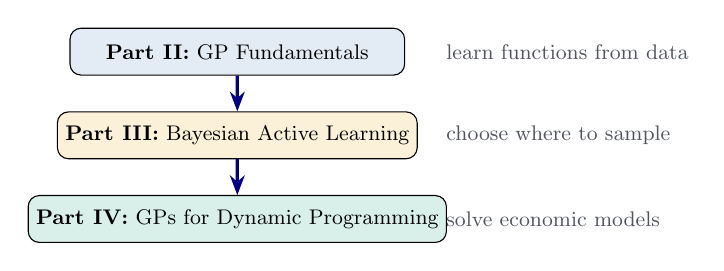
\begin{tikzpicture}[
    box/.style={draw, rounded corners=4pt, minimum width=5cm,
                minimum height=0.7cm, align=center, font=\small},
    arr/.style={-{Stealth[length=2.5mm]}, very thick, uzhblue},
    scale=0.85, transform shape
]
    \node[box, fill=softblue!15] (gp) at (0,2.5) {\textbf{Part II:} GP Fundamentals};
    \node[box, fill=softorange!15] (bal) at (0,1.25) {\textbf{Part III:} Bayesian Active Learning};
    \node[box, fill=softgreen!15] (dp) at (0,0) {\textbf{Part IV:} GPs for Dynamic Programming};

    \draw[arr] (gp) -- (bal);
    \draw[arr] (bal) -- (dp);

    \node[font=\small, text=uzhgreydark, anchor=west] at (3,2.5) {learn functions from data};
    \node[font=\small, text=uzhgreydark, anchor=west] at (3,1.25) {choose where to sample};
    \node[font=\small, text=uzhgreydark, anchor=west] at (3,0) {solve economic models};
\end{tikzpicture}
\end{center}

\vspace{0.4em}
{\small Reference: Scheidegger \& Bilionis (2019), ``Machine Learning for High-Dimensional Dynamic Stochastic Economies,'' \emph{J.\ Computational Science} 33, 68--82.}

\vspace{0.2em}
\begin{block}{Hands-on}
\small \textbf{Notebook:} \texttt{04\_GP\_Value\_Function\_Iteration.ipynb} (in \texttt{day7/code/}).
\end{block}
\end{frame}

% ============================================================================
% PART V: SUMMARY & OUTLOOK
% ============================================================================
\section{Summary \& Outlook}

\begin{frame}{Recap: The Computational Toolbox}
\small
\begin{columns}[T]
\begin{column}{0.24\textwidth}
\begin{block}{\small PINNs}
\scriptsize
\begin{itemize}\itemsep0pt
  \item Continuous-time PDEs
  \item Physics loss
  \item Mesh-free
  \item HJB, Black--Scholes
\end{itemize}
\end{block}
\end{column}
\begin{column}{0.24\textwidth}
\begin{block}{\small Deep Surrogates}
\scriptsize
\begin{itemize}\itemsep0pt
  \item Discrete-time
  \item Pseudo-states
  \item Fast evaluation
  \item Estimation, UQ
\end{itemize}
\end{block}
\end{column}
\begin{column}{0.24\textwidth}
\begin{block}{\small GPs + BAL}
\scriptsize
\begin{itemize}\itemsep0pt
  \item Nonparametric
  \item Built-in UQ
  \item Active learning
  \item Moderate dim
\end{itemize}
\end{block}
\end{column}
\begin{column}{0.24\textwidth}
\begin{block}{\small ASGP + VFI}
\scriptsize
\begin{itemize}\itemsep0pt
  \item GP inside DP
  \item Active Subspaces
  \item Up to 500D
  \item Ergodic sets
\end{itemize}
\end{block}
\end{column}
\end{columns}

\vspace{0.3cm}
All four approaches are \emphc{complementary}: choose based on the problem structure, dimensionality, whether UQ is needed, and available hardware.
\end{frame}

% --- Slide 42: The Toolbox ---
\begin{frame}{The Toolbox: When to Use What}
\begin{center}
\scriptsize
\begin{tabular}{l l l}
\toprule
\textbf{Method} & \textbf{Best for} & \textbf{Key strength} \\
\midrule
\textbf{DEQN} & Discrete-time equilibrium models & Scales to high $d$, Euler eq.\ loss \\
\textbf{PINN} & Continuous-time PDEs/HJB & Mesh-free, physics-constrained \\
\textbf{Deep Surrogate} & Fast evaluation, estimation, UQ & Pseudo-states, autograd \\
\textbf{GP + BAL} & Moderate $d$, need UQ & Built-in uncertainty, active learning \\
\textbf{Deep Kernel} & Warped inputs + need UQ & Learned features + GP uncertainty \\
\bottomrule
\end{tabular}
\end{center}

\vspace{0.15cm}
\begin{block}{Decision heuristic}
\scriptsize
\begin{enumerate}
  \item Is it a continuous-time PDE? $\Rightarrow$ \textbf{PINN}.
  \item Do you need to re-evaluate for many parameter values? $\Rightarrow$ \textbf{Deep Surrogate}.
  \item Is $d \leq 10$ and you need UQ / active learning? $\Rightarrow$ \textbf{GP + BAL}.
  \item Is the latent structure smooth, but the raw input geometry is poor? $\Rightarrow$ \textbf{Deep Kernel}.
  \item Is it a discrete-time equilibrium model? $\Rightarrow$ \textbf{DEQN}.
\end{enumerate}
\end{block}
\end{frame}

% --- Slide 43: References & Questions ---
\begin{frame}[shrink=5]{References \& Resources}
\footnotesize
\textbf{Key papers:}
\begin{itemize}\itemsep0pt \parskip0pt
  \item Chen, Didisheim \& Scheidegger (2026). \emph{Deep Surrogates for Finance: With an Application to Option Pricing.} J.\ Financial Econ.
  \item Scheidegger \& Bilionis (2019). \emph{ML for High-Dim Dynamic Stochastic Economies.} J.\ Comput.\ Sci.
  \item K\"ubler, Scheidegger \& Surbek (2026). \emph{Using Machine Learning to Compute Constrained Optimal Carbon Tax Rules.} Forthcoming in \emph{JPE Macroeconomics}.
  \item Rasmussen \& Williams (2006). \emph{GP for ML.} MIT Press.
  \item Wilson et al.\ (2016). \emph{Deep Kernel Learning.} AISTATS.
\end{itemize}

\vspace{0.1cm}
{\tiny \textbf{Notebooks:} \texttt{01\_Surrogate\_Primer}, \texttt{02\_GP\_and\_BAL}, \texttt{03\_Structural\_Estimation\_BM}, \texttt{04\_GP\_Value\_Function\_Iteration}, \texttt{05--07\_Active\_Subspace} (2D, 10D, nonlinear), \texttt{08\_Deep\_Kernel\_Learning}, \texttt{09\_Deep\_Active\_Subspace\_Ridge}, \texttt{10\_Deep\_AS\_vs\_Linear\_AS\_Borehole}}

\vspace{0.15cm}
\textbf{GitHub:} \url{https://github.com/sischei/Deep_Learning_for_Solving_And_Estimating_Dynamic_Economic_Models}

\vspace{0.2cm}
\begin{center}
{\LARGE \emphc{Questions?}}
\end{center}
\end{frame}

\end{document}
